% 2006 年上海春季卷第 17 题：长方体及题干指定的两条异面直线。
% 只示意原卷可见拓扑与虚实线，不按比例，不暗示边长比例。
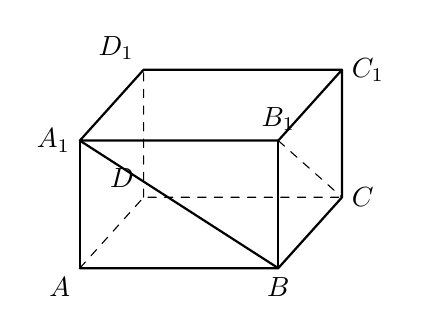
\begin{tikzpicture}[line cap=round,line join=round,scale=0.9]
  \coordinate (A) at (0,0);
  \coordinate (B) at (2.8,0);
  \coordinate (C) at (3.7,1.0);
  \coordinate (D) at (0.9,1.0);
  \coordinate (A1) at (0,1.8);
  \coordinate (B1) at (2.8,1.8);
  \coordinate (C1) at (3.7,2.8);
  \coordinate (D1) at (0.9,2.8);

  % 长方体可见棱与遮挡棱。
  \draw[thick] (A)--(B)--(C)--(C1)--(B1)--(A1)--(D1)--(C1);
  \draw[thick] (A1)--(A) (B1)--(B);
  \draw[dashed] (A)--(D)--(C) (D)--(D1);

  % 题干中的 A_1B 与 B_1C。
  \draw[thick] (A1)--(B);
  \draw[dashed] (B1)--(C);

  \node[below left] at (A) {$A$};
  \node[below] at (B) {$B$};
  \node[right] at (C) {$C$};
  \node[above left] at (D) {$D$};
  \node[left] at (A1) {$A_1$};
  \node[above] at (B1) {$B_1$};
  \node[right] at (C1) {$C_1$};
  \node[above left] at (D1) {$D_1$};
\end{tikzpicture}
